\documentclass[1p]{elsarticle_modified}
%\bibliographystyle{elsarticle-num}

%\usepackage[colorlinks]{hyperref}
%\usepackage{abbrmath_seonhwa} %\Abb, \Ascr, \Acal ,\Abf, \Afrak
\usepackage{amsfonts}
\usepackage{amssymb}
\usepackage{amsmath}
\usepackage{amsthm}
\usepackage{scalefnt}
\usepackage{amsbsy}
\usepackage{kotex}
\usepackage{caption}
\usepackage{subfig}
\usepackage{color}
\usepackage{graphicx}
\usepackage{xcolor} %% white, black, red, green, blue, cyan, magenta, yellow
\usepackage{float}
\usepackage{setspace}
\usepackage{hyperref}

\usepackage{tikz}
\usetikzlibrary{arrows}

\usepackage{multirow}
\usepackage{array} % fixed length table
\usepackage{hhline}

%%%%%%%%%%%%%%%%%%%%%
\makeatletter
\renewcommand*\env@matrix[1][\arraystretch]{%
	\edef\arraystretch{#1}%
	\hskip -\arraycolsep
	\let\@ifnextchar\new@ifnextchar
	\array{*\c@MaxMatrixCols c}}
\makeatother %https://tex.stackexchange.com/questions/14071/how-can-i-increase-the-line-spacing-in-a-matrix
%%%%%%%%%%%%%%%

\usepackage[normalem]{ulem}

\newcommand{\msout}[1]{\ifmmode\text{\sout{\ensuremath{#1}}}\else\sout{#1}\fi}
%SOURCE: \msout is \stkout macro in https://tex.stackexchange.com/questions/20609/strikeout-in-math-mode

\newcommand{\cancel}[1]{
	\ifmmode
	{\color{red}\msout{#1}}
	\else
	{\color{red}\sout{#1}}
	\fi
}

\newcommand{\add}[1]{
	{\color{blue}\uwave{#1}}
}

\newcommand{\replace}[2]{
	\ifmmode
	{\color{red}\msout{#1}}{\color{blue}\uwave{#2}}
	\else
	{\color{red}\sout{#1}}{\color{blue}\uwave{#2}}
	\fi
}

\newcommand{\Sol}{\mathcal{S}} %segment
\newcommand{\D}{D} %diagram
\newcommand{\A}{\mathcal{A}} %arc


%%%%%%%%%%%%%%%%%%%%%%%%%%%%%5 test

\def\sl{\operatorname{\textup{SL}}(2,\Cbb)}
\def\psl{\operatorname{\textup{PSL}}(2,\Cbb)}
\def\quan{\mkern 1mu \triangleright \mkern 1mu}

\theoremstyle{definition}
\newtheorem{thm}{Theorem}[section]
\newtheorem{prop}[thm]{Proposition}
\newtheorem{lem}[thm]{Lemma}
\newtheorem{ques}[thm]{Question}
\newtheorem{cor}[thm]{Corollary}
\newtheorem{defn}[thm]{Definition}
\newtheorem{exam}[thm]{Example}
\newtheorem{rmk}[thm]{Remark}
\newtheorem{alg}[thm]{Algorithm}

\newcommand{\I}{\sqrt{-1}}
\begin{document}

%\begin{frontmatter}
%
%\title{Boundary parabolic representations of knots up to 8 crossings}
%
%%% Group authors per affiliation:
%\author{Yunhi Cho} 
%\address{Department of Mathematics, University of Seoul, Seoul, Korea}
%\ead{yhcho@uos.ac.kr}
%
%
%\author{Seonhwa Kim} %\fnref{s_kim}}
%\address{Center for Geometry and Physics, Institute for Basic Science, Pohang, 37673, Korea}
%\ead{ryeona17@ibs.re.kr}
%
%\author{Hyuk Kim}
%\address{Department of Mathematical Sciences, Seoul National University, Seoul 08826, Korea}
%\ead{hyukkim@snu.ac.kr}
%
%\author{Seokbeom Yoon}
%\address{Department of Mathematical Sciences, Seoul National University, Seoul, 08826,  Korea}
%\ead{sbyoon15@snu.ac.kr}
%
%\begin{abstract}
%We find all boundary parabolic representation of knots up to 8 crossings.
%
%\end{abstract}
%\begin{keyword}
%    \MSC[2010] 57M25 
%\end{keyword}
%
%\end{frontmatter}

%\linenumbers
%\tableofcontents
%
\newcommand\colored[1]{\textcolor{white}{\rule[-0.35ex]{0.8em}{1.4ex}}\kern-0.8em\color{red} #1}%
%\newcommand\colored[1]{\textcolor{white}{ #1}\kern-2.17ex	\textcolor{white}{ #1}\kern-1.81ex	\textcolor{white}{ #1}\kern-2.15ex\color{red}#1	}

{\Large $\underline{12a_{0149}~(K12a_{0149})}$}

\setlength{\tabcolsep}{10pt}
\renewcommand{\arraystretch}{1.6}
\vspace{1cm}\begin{tabular}{m{100pt}>{\centering\arraybackslash}m{274pt}}
\multirow{5}{120pt}{
	\centering
	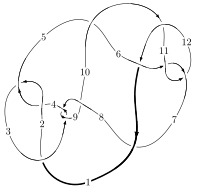
\includegraphics[width=112pt]{../../../GIT/diagram.site/Diagrams/png/950_12a_0149.png}\\
\ \ \ A knot diagram\footnotemark}&
\allowdisplaybreaks
\textbf{Linearized knot diagam} \\
\cline{2-2}
 &
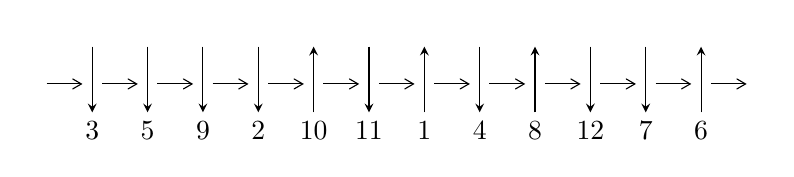
\begin{tikzpicture}[x=20pt, y=17pt]
	% nodes
	\node (C0) at (0, 0) {};
	\node (C1) at (1, 0) {};
	\node (C1U) at (1, +1) {};
	\node (C1D) at (1, -1) {3};

	\node (C2) at (2, 0) {};
	\node (C2U) at (2, +1) {};
	\node (C2D) at (2, -1) {5};

	\node (C3) at (3, 0) {};
	\node (C3U) at (3, +1) {};
	\node (C3D) at (3, -1) {9};

	\node (C4) at (4, 0) {};
	\node (C4U) at (4, +1) {};
	\node (C4D) at (4, -1) {2};

	\node (C5) at (5, 0) {};
	\node (C5U) at (5, +1) {};
	\node (C5D) at (5, -1) {10};

	\node (C6) at (6, 0) {};
	\node (C6U) at (6, +1) {};
	\node (C6D) at (6, -1) {11};

	\node (C7) at (7, 0) {};
	\node (C7U) at (7, +1) {};
	\node (C7D) at (7, -1) {1};

	\node (C8) at (8, 0) {};
	\node (C8U) at (8, +1) {};
	\node (C8D) at (8, -1) {4};

	\node (C9) at (9, 0) {};
	\node (C9U) at (9, +1) {};
	\node (C9D) at (9, -1) {8};

	\node (C10) at (10, 0) {};
	\node (C10U) at (10, +1) {};
	\node (C10D) at (10, -1) {12};

	\node (C11) at (11, 0) {};
	\node (C11U) at (11, +1) {};
	\node (C11D) at (11, -1) {7};

	\node (C12) at (12, 0) {};
	\node (C12U) at (12, +1) {};
	\node (C12D) at (12, -1) {6};
	\node (C13) at (13, 0) {};

	% arrows
	\draw[->,>={angle 60}]
	(C0) edge (C1) (C1) edge (C2) (C2) edge (C3) (C3) edge (C4) (C4) edge (C5) (C5) edge (C6) (C6) edge (C7) (C7) edge (C8) (C8) edge (C9) (C9) edge (C10) (C10) edge (C11) (C11) edge (C12) (C12) edge (C13) ;	\draw[->,>=stealth]
	(C1U) edge (C1D) (C2U) edge (C2D) (C3U) edge (C3D) (C4U) edge (C4D) (C5D) edge (C5U) (C6U) edge (C6D) (C7D) edge (C7U) (C8U) edge (C8D) (C9D) edge (C9U) (C10U) edge (C10D) (C11U) edge (C11D) (C12D) edge (C12U) ;
	\end{tikzpicture} \\
\hhline{~~} \\& 
\textbf{Solving Sequence} \\ \cline{2-2} 
 &
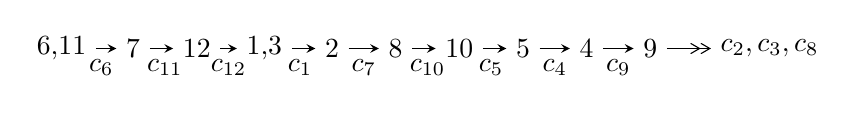
\begin{tikzpicture}[x=23pt, y=7pt]
	% node
	\node (A0) at (-1/8, 0) {6,11};
	\node (A1) at (1, 0) {7};
	\node (A2) at (2, 0) {12};
	\node (A3) at (49/16, 0) {1,3};
	\node (A4) at (33/8, 0) {2};
	\node (A5) at (41/8, 0) {8};
	\node (A6) at (49/8, 0) {10};
	\node (A7) at (57/8, 0) {5};
	\node (A8) at (65/8, 0) {4};
	\node (A9) at (73/8, 0) {9};
	\node (C1) at (1/2, -1) {$c_{6}$};
	\node (C2) at (3/2, -1) {$c_{11}$};
	\node (C3) at (5/2, -1) {$c_{12}$};
	\node (C4) at (29/8, -1) {$c_{1}$};
	\node (C5) at (37/8, -1) {$c_{7}$};
	\node (C6) at (45/8, -1) {$c_{10}$};
	\node (C7) at (53/8, -1) {$c_{5}$};
	\node (C8) at (61/8, -1) {$c_{4}$};
	\node (C9) at (69/8, -1) {$c_{9}$};
	\node (A10) at (11, 0) {$c_{2},c_{3},c_{8}$};

	% edge
	\draw[->,>=stealth]	
	(A0) edge (A1) (A1) edge (A2) (A2) edge (A3) (A3) edge (A4) (A4) edge (A5) (A5) edge (A6) (A6) edge (A7) (A7) edge (A8) (A8) edge (A9) ;
	\draw[->>,>={angle 60}]	
	(A9) edge (A10);
\end{tikzpicture} \\ 

\end{tabular} \\

\footnotetext{
The image of knot diagram is generated by the software ``\textbf{Draw programme}" developed by Andrew Bartholomew(\url{http://www.layer8.co.uk/maths/draw/index.htm\#Running-draw}), where we modified some parts for our purpose(\url{https://github.com/CATsTAILs/LinksPainter}).
}\phantom \\ \newline 
\centering \textbf{Ideals for irreducible components\footnotemark of $X_{\text{par}}$} 
 
\begin{align*}
I^u_{1}&=\langle 
- u^{104}- u^{103}+\cdots+b-2 u,\;- u^{102}- u^{101}+\cdots+a-1,\;u^{105}+2 u^{104}+\cdots+3 u+1\rangle \\
I^u_{2}&=\langle 
b+1,\;- u^4+u^2+a+u,\;u^6+u^5- u^4-2 u^3+u+1\rangle \\
\\
\end{align*}
\raggedright * 2 irreducible components of $\dim_{\mathbb{C}}=0$, with total 111 representations.\\
\footnotetext{All coefficients of polynomials are rational numbers. But the coefficients are sometimes approximated in decimal forms when there is not enough margin.}
\newpage
\renewcommand{\arraystretch}{1}
\centering \section*{I. $I^u_{1}= \langle - u^{104}- u^{103}+\cdots+b-2 u,\;- u^{102}- u^{101}+\cdots+a-1,\;u^{105}+2 u^{104}+\cdots+3 u+1 \rangle$}
\flushleft \textbf{(i) Arc colorings}\\
\begin{tabular}{m{7pt} m{180pt} m{7pt} m{180pt} }
\flushright $a_{6}=$&$\begin{pmatrix}1\\0\end{pmatrix}$ \\
\flushright $a_{11}=$&$\begin{pmatrix}0\\u\end{pmatrix}$ \\
\flushright $a_{7}=$&$\begin{pmatrix}1\\u^2\end{pmatrix}$ \\
\flushright $a_{12}=$&$\begin{pmatrix}- u\\- u^3+u\end{pmatrix}$ \\
\flushright $a_{1}=$&$\begin{pmatrix}- u^3\\- u^3+u\end{pmatrix}$ \\
\flushright $a_{3}=$&$\begin{pmatrix}u^{102}+u^{101}+\cdots-5 u+1\\u^{104}+u^{103}+\cdots-2 u^2+2 u\end{pmatrix}$ \\
\flushright $a_{2}=$&$\begin{pmatrix}- u^{104}- u^{103}+\cdots+6 u^2-5 u\\u^{104}+u^{103}+\cdots- u^2+3 u\end{pmatrix}$ \\
\flushright $a_{8}=$&$\begin{pmatrix}u^8- u^6+u^4+1\\u^8-2 u^6+2 u^4\end{pmatrix}$ \\
\flushright $a_{10}=$&$\begin{pmatrix}u^3\\u^5- u^3+u\end{pmatrix}$ \\
\flushright $a_{5}=$&$\begin{pmatrix}u^8- u^6+u^4+1\\u^{10}-2 u^8+3 u^6-2 u^4+u^2\end{pmatrix}$ \\
\flushright $a_{4}=$&$\begin{pmatrix}-2 u^{104}-2 u^{103}+\cdots+8 u^2-7 u\\u^{104}+u^{103}+\cdots-12 u^3+3 u\end{pmatrix}$ \\
\flushright $a_{9}=$&$\begin{pmatrix}- u^{21}+4 u^{19}+\cdots+2 u^3- u\\- u^{21}+5 u^{19}-13 u^{17}+20 u^{15}-20 u^{13}+13 u^{11}-7 u^9+4 u^7- u^5- u^3+u\end{pmatrix}$\\&\end{tabular}
\flushleft \textbf{(ii) Obstruction class $= -1$}\\~\\
\flushleft \textbf{(iii) Cusp Shapes $= -2 u^{103}+47 u^{101}+\cdots+4 u-10$}\\~\\
\newpage\renewcommand{\arraystretch}{1}
\flushleft \textbf{(iv) u-Polynomials at the component}\newline \\
\begin{tabular}{m{50pt}|m{274pt}}
Crossings & \hspace{64pt}u-Polynomials at each crossing \\
\hline $$\begin{aligned}c_{1}\end{aligned}$$&$\begin{aligned}
&u^{105}+55 u^{104}+\cdots+8 u+1
\end{aligned}$\\
\hline $$\begin{aligned}c_{2},c_{4}\end{aligned}$$&$\begin{aligned}
&u^{105}-7 u^{104}+\cdots-6 u+1
\end{aligned}$\\
\hline $$\begin{aligned}c_{3},c_{8}\end{aligned}$$&$\begin{aligned}
&u^{105}- u^{104}+\cdots+64 u+64
\end{aligned}$\\
\hline $$\begin{aligned}c_{5},c_{7}\end{aligned}$$&$\begin{aligned}
&u^{105}-2 u^{104}+\cdots+333 u+9
\end{aligned}$\\
\hline $$\begin{aligned}c_{6},c_{11}\end{aligned}$$&$\begin{aligned}
&u^{105}+2 u^{104}+\cdots+3 u+1
\end{aligned}$\\
\hline $$\begin{aligned}c_{9}\end{aligned}$$&$\begin{aligned}
&u^{105}-39 u^{104}+\cdots-81920 u+4096
\end{aligned}$\\
\hline $$\begin{aligned}c_{10}\end{aligned}$$&$\begin{aligned}
&u^{105}+48 u^{104}+\cdots+15 u+1
\end{aligned}$\\
\hline $$\begin{aligned}c_{12}\end{aligned}$$&$\begin{aligned}
&u^{105}+6 u^{104}+\cdots+99 u+5
\end{aligned}$\\
\hline
\end{tabular}\\~\\
\newpage\renewcommand{\arraystretch}{1}
\flushleft \textbf{(v) Riley Polynomials at the component}\newline \\
\begin{tabular}{m{50pt}|m{274pt}}
Crossings & \hspace{64pt}Riley Polynomials at each crossing \\
\hline $$\begin{aligned}c_{1}\end{aligned}$$&$\begin{aligned}
&y^{105}-3 y^{104}+\cdots-8 y-1
\end{aligned}$\\
\hline $$\begin{aligned}c_{2},c_{4}\end{aligned}$$&$\begin{aligned}
&y^{105}-55 y^{104}+\cdots+8 y-1
\end{aligned}$\\
\hline $$\begin{aligned}c_{3},c_{8}\end{aligned}$$&$\begin{aligned}
&y^{105}+39 y^{104}+\cdots-81920 y-4096
\end{aligned}$\\
\hline $$\begin{aligned}c_{5},c_{7}\end{aligned}$$&$\begin{aligned}
&y^{105}-72 y^{104}+\cdots+23067 y-81
\end{aligned}$\\
\hline $$\begin{aligned}c_{6},c_{11}\end{aligned}$$&$\begin{aligned}
&y^{105}-48 y^{104}+\cdots+15 y-1
\end{aligned}$\\
\hline $$\begin{aligned}c_{9}\end{aligned}$$&$\begin{aligned}
&y^{105}+43 y^{104}+\cdots+486539264 y-16777216
\end{aligned}$\\
\hline $$\begin{aligned}c_{10}\end{aligned}$$&$\begin{aligned}
&y^{105}+20 y^{104}+\cdots+143 y-1
\end{aligned}$\\
\hline $$\begin{aligned}c_{12}\end{aligned}$$&$\begin{aligned}
&y^{105}+8 y^{104}+\cdots-29 y-25
\end{aligned}$\\
\hline
\end{tabular}\\~\\
\newpage\flushleft \textbf{(vi) Complex Volumes and Cusp Shapes}
$$\begin{array}{c|c|c}  
\text{Solutions to }I^u_{1}& \I (\text{vol} + \sqrt{-1}CS) & \text{Cusp shape}\\
 \hline 
\begin{aligned}
u &= \phantom{-}0.871041 + 0.511708 I \\
a &= -0.369393 - 0.110166 I \\
b &= \phantom{-}0.440206 - 0.618461 I\end{aligned}
 & \phantom{-}1.88999 - 2.94964 I & \phantom{-0.000000 } 0 \\ \hline\begin{aligned}
u &= \phantom{-}0.871041 - 0.511708 I \\
a &= -0.369393 + 0.110166 I \\
b &= \phantom{-}0.440206 + 0.618461 I\end{aligned}
 & \phantom{-}1.88999 + 2.94964 I & \phantom{-0.000000 } 0 \\ \hline\begin{aligned}
u &= \phantom{-}0.922799 + 0.352325 I \\
a &= -1.77246 + 0.60448 I \\
b &= -1.312370 + 0.212834 I\end{aligned}
 & -2.93812 - 1.40462 I & \phantom{-0.000000 } 0 \\ \hline\begin{aligned}
u &= \phantom{-}0.922799 - 0.352325 I \\
a &= -1.77246 - 0.60448 I \\
b &= -1.312370 - 0.212834 I\end{aligned}
 & -2.93812 + 1.40462 I & \phantom{-0.000000 } 0 \\ \hline\begin{aligned}
u &= -0.921835 + 0.433717 I \\
a &= -1.18386 - 2.01805 I \\
b &= -1.236050 + 0.589796 I\end{aligned}
 & -2.05807 + 3.12857 I & \phantom{-0.000000 } 0 \\ \hline\begin{aligned}
u &= -0.921835 - 0.433717 I \\
a &= -1.18386 + 2.01805 I \\
b &= -1.236050 - 0.589796 I\end{aligned}
 & -2.05807 - 3.12857 I & \phantom{-0.000000 } 0 \\ \hline\begin{aligned}
u &= -1.020100 + 0.189153 I \\
a &= \phantom{-}0.430373 - 1.257180 I \\
b &= -0.437411 - 0.526557 I\end{aligned}
 & -1.85386 + 0.21349 I & \phantom{-0.000000 } 0 \\ \hline\begin{aligned}
u &= -1.020100 - 0.189153 I \\
a &= \phantom{-}0.430373 + 1.257180 I \\
b &= -0.437411 + 0.526557 I\end{aligned}
 & -1.85386 - 0.21349 I & \phantom{-0.000000 } 0 \\ \hline\begin{aligned}
u &= \phantom{-}1.058570 + 0.031241 I \\
a &= -0.73900 + 2.50720 I \\
b &= -0.281684 + 1.135380 I\end{aligned}
 & \phantom{-}2.93779 + 2.55382 I & \phantom{-0.000000 } 0 \\ \hline\begin{aligned}
u &= \phantom{-}1.058570 - 0.031241 I \\
a &= -0.73900 - 2.50720 I \\
b &= -0.281684 - 1.135380 I\end{aligned}
 & \phantom{-}2.93779 - 2.55382 I & \phantom{-0.000000 } 0\\
 \hline 
 \end{array}$$\newpage$$\begin{array}{c|c|c}  
\text{Solutions to }I^u_{1}& \I (\text{vol} + \sqrt{-1}CS) & \text{Cusp shape}\\
 \hline 
\begin{aligned}
u &= \phantom{-}0.921723 + 0.557628 I \\
a &= \phantom{-}1.06654 - 1.37317 I \\
b &= \phantom{-}0.838100 + 0.698342 I\end{aligned}
 & \phantom{-}0.10374 - 7.55958 I & \phantom{-0.000000 } 0 \\ \hline\begin{aligned}
u &= \phantom{-}0.921723 - 0.557628 I \\
a &= \phantom{-}1.06654 + 1.37317 I \\
b &= \phantom{-}0.838100 - 0.698342 I\end{aligned}
 & \phantom{-}0.10374 + 7.55958 I & \phantom{-0.000000 } 0 \\ \hline\begin{aligned}
u &= -0.561631 + 0.730673 I \\
a &= \phantom{-}0.317415 + 0.482062 I \\
b &= \phantom{-}0.44589 + 2.35840 I\end{aligned}
 & \phantom{-}3.08653 + 9.35903 I & \phantom{-0.000000 } 0 \\ \hline\begin{aligned}
u &= -0.561631 - 0.730673 I \\
a &= \phantom{-}0.317415 - 0.482062 I \\
b &= \phantom{-}0.44589 - 2.35840 I\end{aligned}
 & \phantom{-}3.08653 - 9.35903 I & \phantom{-0.000000 } 0 \\ \hline\begin{aligned}
u &= \phantom{-}1.068320 + 0.168089 I \\
a &= -1.99637 - 0.28617 I \\
b &= -1.55455 - 0.55344 I\end{aligned}
 & -4.75936 + 1.13660 I & \phantom{-0.000000 } 0 \\ \hline\begin{aligned}
u &= \phantom{-}1.068320 - 0.168089 I \\
a &= -1.99637 + 0.28617 I \\
b &= -1.55455 + 0.55344 I\end{aligned}
 & -4.75936 - 1.13660 I & \phantom{-0.000000 } 0 \\ \hline\begin{aligned}
u &= -0.541684 + 0.731152 I \\
a &= -0.571433 - 0.349082 I \\
b &= -0.625316 - 0.742225 I\end{aligned}
 & \phantom{-}5.63434 + 4.07144 I & \phantom{-0.000000 } 0 \\ \hline\begin{aligned}
u &= -0.541684 - 0.731152 I \\
a &= -0.571433 + 0.349082 I \\
b &= -0.625316 + 0.742225 I\end{aligned}
 & \phantom{-}5.63434 - 4.07144 I & \phantom{-0.000000 } 0 \\ \hline\begin{aligned}
u &= -1.082220 + 0.152274 I \\
a &= \phantom{-}1.05559 + 3.81169 I \\
b &= \phantom{-}1.45512 + 1.53677 I\end{aligned}
 & -4.31563 - 3.76778 I & \phantom{-0.000000 } 0 \\ \hline\begin{aligned}
u &= -1.082220 - 0.152274 I \\
a &= \phantom{-}1.05559 - 3.81169 I \\
b &= \phantom{-}1.45512 - 1.53677 I\end{aligned}
 & -4.31563 + 3.76778 I & \phantom{-0.000000 } 0\\
 \hline 
 \end{array}$$\newpage$$\begin{array}{c|c|c}  
\text{Solutions to }I^u_{1}& \I (\text{vol} + \sqrt{-1}CS) & \text{Cusp shape}\\
 \hline 
\begin{aligned}
u &= -0.491163 + 0.760253 I \\
a &= -0.303412 + 0.316758 I \\
b &= \phantom{-}0.02554 + 2.32363 I\end{aligned}
 & \phantom{-}8.31059 + 1.25002 I & \phantom{-0.000000 } 0 \\ \hline\begin{aligned}
u &= -0.491163 - 0.760253 I \\
a &= -0.303412 - 0.316758 I \\
b &= \phantom{-}0.02554 - 2.32363 I\end{aligned}
 & \phantom{-}8.31059 - 1.25002 I & \phantom{-0.000000 } 0 \\ \hline\begin{aligned}
u &= -0.468964 + 0.768998 I \\
a &= -0.234001 - 0.389085 I \\
b &= -1.11862 - 1.92816 I\end{aligned}
 & \phantom{-}8.18758 - 4.15070 I & \phantom{-0.000000 } 0 \\ \hline\begin{aligned}
u &= -0.468964 - 0.768998 I \\
a &= -0.234001 + 0.389085 I \\
b &= -1.11862 + 1.92816 I\end{aligned}
 & \phantom{-}8.18758 + 4.15070 I & \phantom{-0.000000 } 0 \\ \hline\begin{aligned}
u &= \phantom{-}1.094480 + 0.131917 I \\
a &= -0.02662 - 1.62635 I \\
b &= \phantom{-}0.647265 - 0.798129 I\end{aligned}
 & -0.04159 + 4.70125 I & \phantom{-0.000000 } 0 \\ \hline\begin{aligned}
u &= \phantom{-}1.094480 - 0.131917 I \\
a &= -0.02662 + 1.62635 I \\
b &= \phantom{-}0.647265 + 0.798129 I\end{aligned}
 & -0.04159 - 4.70125 I & \phantom{-0.000000 } 0 \\ \hline\begin{aligned}
u &= -1.061330 + 0.302887 I \\
a &= \phantom{-}0.650283 - 0.216021 I \\
b &= \phantom{-}0.161826 - 0.038082 I\end{aligned}
 & -2.49722 + 0.52024 I & \phantom{-0.000000 } 0 \\ \hline\begin{aligned}
u &= -1.061330 - 0.302887 I \\
a &= \phantom{-}0.650283 + 0.216021 I \\
b &= \phantom{-}0.161826 + 0.038082 I\end{aligned}
 & -2.49722 - 0.52024 I & \phantom{-0.000000 } 0 \\ \hline\begin{aligned}
u &= \phantom{-}0.535147 + 0.710912 I \\
a &= -0.144639 + 0.767528 I \\
b &= -0.49756 + 2.66326 I\end{aligned}
 & \phantom{-}1.20196 - 3.31272 I & \phantom{-0.000000 -}0. + 4.05275 I \\ \hline\begin{aligned}
u &= \phantom{-}0.535147 - 0.710912 I \\
a &= -0.144639 - 0.767528 I \\
b &= -0.49756 - 2.66326 I\end{aligned}
 & \phantom{-}1.20196 + 3.31272 I & \phantom{-0.000000 } 0. - 4.05275 I\\
 \hline 
 \end{array}$$\newpage$$\begin{array}{c|c|c}  
\text{Solutions to }I^u_{1}& \I (\text{vol} + \sqrt{-1}CS) & \text{Cusp shape}\\
 \hline 
\begin{aligned}
u &= -0.407168 + 0.786367 I \\
a &= \phantom{-}0.366623 - 0.319641 I \\
b &= -0.93186 - 3.09556 I\end{aligned}
 & \phantom{-}2.24833 - 12.15740 I & \phantom{-0.000000 -}0. + 7.45112 I \\ \hline\begin{aligned}
u &= -0.407168 - 0.786367 I \\
a &= \phantom{-}0.366623 + 0.319641 I \\
b &= -0.93186 + 3.09556 I\end{aligned}
 & \phantom{-}2.24833 + 12.15740 I & \phantom{-0.000000 } 0. - 7.45112 I \\ \hline\begin{aligned}
u &= -0.418533 + 0.777892 I \\
a &= -0.565706 + 0.154413 I \\
b &= \phantom{-}0.12298 + 1.64263 I\end{aligned}
 & \phantom{-}4.96689 - 6.83862 I & \phantom{-0.000000 -}0. + 4.01071 I \\ \hline\begin{aligned}
u &= -0.418533 - 0.777892 I \\
a &= -0.565706 - 0.154413 I \\
b &= \phantom{-}0.12298 - 1.64263 I\end{aligned}
 & \phantom{-}4.96689 + 6.83862 I & \phantom{-0.000000 } 0. - 4.01071 I \\ \hline\begin{aligned}
u &= -1.098480 + 0.220916 I \\
a &= \phantom{-}1.82717 - 0.51460 I \\
b &= \phantom{-}1.28934 - 0.84992 I\end{aligned}
 & -4.64089 + 3.53476 I & \phantom{-0.000000 } 0 \\ \hline\begin{aligned}
u &= -1.098480 - 0.220916 I \\
a &= \phantom{-}1.82717 + 0.51460 I \\
b &= \phantom{-}1.28934 + 0.84992 I\end{aligned}
 & -4.64089 - 3.53476 I & \phantom{-0.000000 } 0 \\ \hline\begin{aligned}
u &= \phantom{-}1.114790 + 0.141950 I \\
a &= -0.62179 + 3.70068 I \\
b &= -1.22790 + 1.88592 I\end{aligned}
 & -2.78241 + 9.87820 I & \phantom{-0.000000 } 0 \\ \hline\begin{aligned}
u &= \phantom{-}1.114790 - 0.141950 I \\
a &= -0.62179 - 3.70068 I \\
b &= -1.22790 - 1.88592 I\end{aligned}
 & -2.78241 - 9.87820 I & \phantom{-0.000000 } 0 \\ \hline\begin{aligned}
u &= \phantom{-}0.412854 + 0.764891 I \\
a &= -0.329970 - 0.580550 I \\
b &= \phantom{-}1.34712 - 3.14233 I\end{aligned}
 & \phantom{-}0.54594 + 5.90508 I & -2.83942 - 4.16325 I \\ \hline\begin{aligned}
u &= \phantom{-}0.412854 - 0.764891 I \\
a &= -0.329970 + 0.580550 I \\
b &= \phantom{-}1.34712 + 3.14233 I\end{aligned}
 & \phantom{-}0.54594 - 5.90508 I & -2.83942 + 4.16325 I\\
 \hline 
 \end{array}$$\newpage$$\begin{array}{c|c|c}  
\text{Solutions to }I^u_{1}& \I (\text{vol} + \sqrt{-1}CS) & \text{Cusp shape}\\
 \hline 
\begin{aligned}
u &= -0.519162 + 0.696598 I \\
a &= \phantom{-}0.639391 + 0.295863 I \\
b &= -1.153370 - 0.377703 I\end{aligned}
 & \phantom{-}0.550091 + 0.784462 I & -1.20480 - 3.39624 I \\ \hline\begin{aligned}
u &= -0.519162 - 0.696598 I \\
a &= \phantom{-}0.639391 - 0.295863 I \\
b &= -1.153370 + 0.377703 I\end{aligned}
 & \phantom{-}0.550091 - 0.784462 I & -1.20480 + 3.39624 I \\ \hline\begin{aligned}
u &= \phantom{-}0.616023 + 0.610806 I \\
a &= -0.618330 + 0.417161 I \\
b &= \phantom{-}0.781913 - 0.579529 I\end{aligned}
 & \phantom{-}0.97348 + 2.95222 I & \phantom{-0.000000 } 0. - 2.99817 I \\ \hline\begin{aligned}
u &= \phantom{-}0.616023 - 0.610806 I \\
a &= -0.618330 - 0.417161 I \\
b &= \phantom{-}0.781913 + 0.579529 I\end{aligned}
 & \phantom{-}0.97348 - 2.95222 I & \phantom{-0.000000 -}0. + 2.99817 I \\ \hline\begin{aligned}
u &= \phantom{-}0.487231 + 0.710886 I \\
a &= \phantom{-}0.568469 - 0.441572 I \\
b &= \phantom{-}1.46675 - 0.61446 I\end{aligned}
 & \phantom{-}3.00709 + 0.79659 I & \phantom{-}0.79816 - 1.47644 I \\ \hline\begin{aligned}
u &= \phantom{-}0.487231 - 0.710886 I \\
a &= \phantom{-}0.568469 + 0.441572 I \\
b &= \phantom{-}1.46675 + 0.61446 I\end{aligned}
 & \phantom{-}3.00709 - 0.79659 I & \phantom{-}0.79816 + 1.47644 I \\ \hline\begin{aligned}
u &= -0.826365 + 0.242657 I \\
a &= \phantom{-}1.77436 + 0.19357 I \\
b &= -0.099112 - 0.575729 I\end{aligned}
 & -1.346980 + 0.143898 I & -5.19438 + 1.02775 I \\ \hline\begin{aligned}
u &= -0.826365 - 0.242657 I \\
a &= \phantom{-}1.77436 - 0.19357 I \\
b &= -0.099112 + 0.575729 I\end{aligned}
 & -1.346980 - 0.143898 I & -5.19438 - 1.02775 I \\ \hline\begin{aligned}
u &= \phantom{-}0.694568 + 0.503832 I \\
a &= \phantom{-}0.426503 - 1.004340 I \\
b &= \phantom{-}0.599221 + 0.208369 I\end{aligned}
 & \phantom{-}2.38068 - 1.26624 I & \phantom{-}3.02682 + 3.59787 I \\ \hline\begin{aligned}
u &= \phantom{-}0.694568 - 0.503832 I \\
a &= \phantom{-}0.426503 + 1.004340 I \\
b &= \phantom{-}0.599221 - 0.208369 I\end{aligned}
 & \phantom{-}2.38068 + 1.26624 I & \phantom{-}3.02682 - 3.59787 I\\
 \hline 
 \end{array}$$\newpage$$\begin{array}{c|c|c}  
\text{Solutions to }I^u_{1}& \I (\text{vol} + \sqrt{-1}CS) & \text{Cusp shape}\\
 \hline 
\begin{aligned}
u &= -0.412674 + 0.751967 I \\
a &= \phantom{-}0.608113 - 0.004611 I \\
b &= -1.42040 + 0.15308 I\end{aligned}
 & -0.02506 - 3.23562 I & -2.54395 + 3.48237 I \\ \hline\begin{aligned}
u &= -0.412674 - 0.751967 I \\
a &= \phantom{-}0.608113 + 0.004611 I \\
b &= -1.42040 - 0.15308 I\end{aligned}
 & -0.02506 + 3.23562 I & -2.54395 - 3.48237 I \\ \hline\begin{aligned}
u &= \phantom{-}0.431391 + 0.735763 I \\
a &= \phantom{-}0.600136 + 0.213703 I \\
b &= \phantom{-}0.42753 + 1.64026 I\end{aligned}
 & \phantom{-}2.71628 + 1.63531 I & \phantom{-0.000000 -}     -6
0. 10   + 0.426013 I \\ \hline\begin{aligned}
u &= \phantom{-}0.431391 - 0.735763 I \\
a &= \phantom{-}0.600136 - 0.213703 I \\
b &= \phantom{-}0.42753 - 1.64026 I\end{aligned}
 & \phantom{-}2.71628 - 1.63531 I & \phantom{-0.000000 }      -6
0. 10   - 0.426013 I \\ \hline\begin{aligned}
u &= -1.085710 + 0.396654 I \\
a &= \phantom{-}0.82643 - 1.17997 I \\
b &= -0.296620 - 1.185670 I\end{aligned}
 & -3.45140 + 1.18279 I & \phantom{-0.000000 } 0 \\ \hline\begin{aligned}
u &= -1.085710 - 0.396654 I \\
a &= \phantom{-}0.82643 + 1.17997 I \\
b &= -0.296620 + 1.185670 I\end{aligned}
 & -3.45140 - 1.18279 I & \phantom{-0.000000 } 0 \\ \hline\begin{aligned}
u &= \phantom{-}1.095630 + 0.417910 I \\
a &= -0.02770 + 1.67149 I \\
b &= -0.70591 + 1.70291 I\end{aligned}
 & -6.99423 - 2.34770 I & \phantom{-0.000000 } 0 \\ \hline\begin{aligned}
u &= \phantom{-}1.095630 - 0.417910 I \\
a &= -0.02770 - 1.67149 I \\
b &= -0.70591 - 1.70291 I\end{aligned}
 & -6.99423 + 2.34770 I & \phantom{-0.000000 } 0 \\ \hline\begin{aligned}
u &= -1.098070 + 0.430864 I \\
a &= -1.50322 + 0.79462 I \\
b &= \phantom{-}0.50933 + 1.51246 I\end{aligned}
 & -6.90518 + 5.01473 I & \phantom{-0.000000 } 0 \\ \hline\begin{aligned}
u &= -1.098070 - 0.430864 I \\
a &= -1.50322 - 0.79462 I \\
b &= \phantom{-}0.50933 - 1.51246 I\end{aligned}
 & -6.90518 - 5.01473 I & \phantom{-0.000000 } 0\\
 \hline 
 \end{array}$$\newpage$$\begin{array}{c|c|c}  
\text{Solutions to }I^u_{1}& \I (\text{vol} + \sqrt{-1}CS) & \text{Cusp shape}\\
 \hline 
\begin{aligned}
u &= -1.116490 + 0.392750 I \\
a &= -0.304426 + 1.186820 I \\
b &= \phantom{-}0.17668 + 1.56892 I\end{aligned}
 & -6.38577 - 3.12199 I & \phantom{-0.000000 } 0 \\ \hline\begin{aligned}
u &= -1.116490 - 0.392750 I \\
a &= -0.304426 - 1.186820 I \\
b &= \phantom{-}0.17668 - 1.56892 I\end{aligned}
 & -6.38577 + 3.12199 I & \phantom{-0.000000 } 0 \\ \hline\begin{aligned}
u &= \phantom{-}0.358533 + 0.732179 I \\
a &= -0.473671 - 0.115244 I \\
b &= \phantom{-}1.248310 + 0.417986 I\end{aligned}
 & -0.180213 - 1.053090 I & -2.77562 + 3.65050 I \\ \hline\begin{aligned}
u &= \phantom{-}0.358533 - 0.732179 I \\
a &= -0.473671 + 0.115244 I \\
b &= \phantom{-}1.248310 - 0.417986 I\end{aligned}
 & -0.180213 + 1.053090 I & -2.77562 - 3.65050 I \\ \hline\begin{aligned}
u &= \phantom{-}1.097470 + 0.449471 I \\
a &= -0.57663 - 1.39142 I \\
b &= \phantom{-}0.655892 - 1.218070 I\end{aligned}
 & -3.08812 - 6.11758 I & \phantom{-0.000000 } 0 \\ \hline\begin{aligned}
u &= \phantom{-}1.097470 - 0.449471 I \\
a &= -0.57663 + 1.39142 I \\
b &= \phantom{-}0.655892 + 1.218070 I\end{aligned}
 & -3.08812 + 6.11758 I & \phantom{-0.000000 } 0 \\ \hline\begin{aligned}
u &= -1.014830 + 0.615237 I \\
a &= \phantom{-}3.24068 - 0.49048 I \\
b &= \phantom{-}1.02632 - 1.84070 I\end{aligned}
 & \phantom{-}1.74031 - 4.22648 I & \phantom{-0.000000 } 0 \\ \hline\begin{aligned}
u &= -1.014830 - 0.615237 I \\
a &= \phantom{-}3.24068 + 0.49048 I \\
b &= \phantom{-}1.02632 + 1.84070 I\end{aligned}
 & \phantom{-}1.74031 + 4.22648 I & \phantom{-0.000000 } 0 \\ \hline\begin{aligned}
u &= \phantom{-}1.028950 + 0.594658 I \\
a &= -3.74068 - 0.70363 I \\
b &= -1.39258 - 2.26144 I\end{aligned}
 & -0.26335 - 1.69761 I & \phantom{-0.000000 } 0 \\ \hline\begin{aligned}
u &= \phantom{-}1.028950 - 0.594658 I \\
a &= -3.74068 + 0.70363 I \\
b &= -1.39258 + 2.26144 I\end{aligned}
 & -0.26335 + 1.69761 I & \phantom{-0.000000 } 0\\
 \hline 
 \end{array}$$\newpage$$\begin{array}{c|c|c}  
\text{Solutions to }I^u_{1}& \I (\text{vol} + \sqrt{-1}CS) & \text{Cusp shape}\\
 \hline 
\begin{aligned}
u &= -1.038610 + 0.583357 I \\
a &= -0.86698 - 1.45055 I \\
b &= -1.123260 + 0.479159 I\end{aligned}
 & -0.99128 + 4.14969 I & \phantom{-0.000000 } 0 \\ \hline\begin{aligned}
u &= -1.038610 - 0.583357 I \\
a &= -0.86698 + 1.45055 I \\
b &= -1.123260 - 0.479159 I\end{aligned}
 & -0.99128 - 4.14969 I & \phantom{-0.000000 } 0 \\ \hline\begin{aligned}
u &= -1.028780 + 0.610157 I \\
a &= -1.38935 - 0.41725 I \\
b &= -0.846242 + 0.238296 I\end{aligned}
 & \phantom{-}4.18740 + 1.04548 I & \phantom{-0.000000 } 0 \\ \hline\begin{aligned}
u &= -1.028780 - 0.610157 I \\
a &= -1.38935 + 0.41725 I \\
b &= -0.846242 - 0.238296 I\end{aligned}
 & \phantom{-}4.18740 - 1.04548 I & \phantom{-0.000000 } 0 \\ \hline\begin{aligned}
u &= \phantom{-}1.119170 + 0.448157 I \\
a &= \phantom{-}0.916526 + 0.862413 I \\
b &= -0.82229 + 1.15840 I\end{aligned}
 & -6.01436 - 10.76980 I & \phantom{-0.000000 } 0 \\ \hline\begin{aligned}
u &= \phantom{-}1.119170 - 0.448157 I \\
a &= \phantom{-}0.916526 - 0.862413 I \\
b &= -0.82229 - 1.15840 I\end{aligned}
 & -6.01436 + 10.76980 I & \phantom{-0.000000 } 0 \\ \hline\begin{aligned}
u &= \phantom{-}1.085540 + 0.531264 I \\
a &= \phantom{-}0.218413 - 0.818317 I \\
b &= \phantom{-}0.272318 - 0.133470 I\end{aligned}
 & -0.96342 - 6.54782 I & \phantom{-0.000000 } 0 \\ \hline\begin{aligned}
u &= \phantom{-}1.085540 - 0.531264 I \\
a &= \phantom{-}0.218413 + 0.818317 I \\
b &= \phantom{-}0.272318 + 0.133470 I\end{aligned}
 & -0.96342 + 6.54782 I & \phantom{-0.000000 } 0 \\ \hline\begin{aligned}
u &= \phantom{-}1.056750 + 0.588724 I \\
a &= \phantom{-}1.89469 - 1.62052 I \\
b &= \phantom{-}1.88122 + 0.04481 I\end{aligned}
 & \phantom{-}1.32189 - 5.78784 I & \phantom{-0.000000 } 0 \\ \hline\begin{aligned}
u &= \phantom{-}1.056750 - 0.588724 I \\
a &= \phantom{-}1.89469 + 1.62052 I \\
b &= \phantom{-}1.88122 - 0.04481 I\end{aligned}
 & \phantom{-}1.32189 + 5.78784 I & \phantom{-0.000000 } 0\\
 \hline 
 \end{array}$$\newpage$$\begin{array}{c|c|c}  
\text{Solutions to }I^u_{1}& \I (\text{vol} + \sqrt{-1}CS) & \text{Cusp shape}\\
 \hline 
\begin{aligned}
u &= -1.064960 + 0.613127 I \\
a &= \phantom{-}2.78431 - 1.21297 I \\
b &= \phantom{-}0.56806 - 2.38367 I\end{aligned}
 & \phantom{-}6.60470 + 3.95245 I & \phantom{-0.000000 } 0 \\ \hline\begin{aligned}
u &= -1.064960 - 0.613127 I \\
a &= \phantom{-}2.78431 + 1.21297 I \\
b &= \phantom{-}0.56806 + 2.38367 I\end{aligned}
 & \phantom{-}6.60470 - 3.95245 I & \phantom{-0.000000 } 0 \\ \hline\begin{aligned}
u &= \phantom{-}1.087140 + 0.587148 I \\
a &= -1.72430 - 1.55120 I \\
b &= -0.06084 - 2.05367 I\end{aligned}
 & \phantom{-}0.78044 - 6.68037 I & \phantom{-0.000000 } 0 \\ \hline\begin{aligned}
u &= \phantom{-}1.087140 - 0.587148 I \\
a &= -1.72430 + 1.55120 I \\
b &= -0.06084 + 2.05367 I\end{aligned}
 & \phantom{-}0.78044 + 6.68037 I & \phantom{-0.000000 } 0 \\ \hline\begin{aligned}
u &= -1.078250 + 0.611228 I \\
a &= -3.10524 - 0.23085 I \\
b &= -1.56999 + 1.66367 I\end{aligned}
 & \phantom{-}6.37670 + 9.36798 I & \phantom{-0.000000 } 0 \\ \hline\begin{aligned}
u &= -1.078250 - 0.611228 I \\
a &= -3.10524 + 0.23085 I \\
b &= -1.56999 - 1.66367 I\end{aligned}
 & \phantom{-}6.37670 - 9.36798 I & \phantom{-0.000000 } 0 \\ \hline\begin{aligned}
u &= \phantom{-}1.107430 + 0.568255 I \\
a &= \phantom{-}0.32467 - 1.75043 I \\
b &= \phantom{-}1.47140 - 0.35337 I\end{aligned}
 & -2.36349 - 3.89444 I & \phantom{-0.000000 } 0 \\ \hline\begin{aligned}
u &= \phantom{-}1.107430 - 0.568255 I \\
a &= \phantom{-}0.32467 + 1.75043 I \\
b &= \phantom{-}1.47140 + 0.35337 I\end{aligned}
 & -2.36349 + 3.89444 I & \phantom{-0.000000 } 0 \\ \hline\begin{aligned}
u &= -1.097390 + 0.588994 I \\
a &= -0.54573 - 1.77669 I \\
b &= -1.57950 - 0.02613 I\end{aligned}
 & -2.04553 + 8.32422 I & \phantom{-0.000000 } 0 \\ \hline\begin{aligned}
u &= -1.097390 - 0.588994 I \\
a &= -0.54573 + 1.77669 I \\
b &= -1.57950 + 0.02613 I\end{aligned}
 & -2.04553 - 8.32422 I & \phantom{-0.000000 } 0\\
 \hline 
 \end{array}$$\newpage$$\begin{array}{c|c|c}  
\text{Solutions to }I^u_{1}& \I (\text{vol} + \sqrt{-1}CS) & \text{Cusp shape}\\
 \hline 
\begin{aligned}
u &= \phantom{-}1.100740 + 0.593524 I \\
a &= \phantom{-}4.65152 + 0.60219 I \\
b &= \phantom{-}2.08615 + 3.31083 I\end{aligned}
 & -1.48870 - 11.04220 I & \phantom{-0.000000 } 0 \\ \hline\begin{aligned}
u &= \phantom{-}1.100740 - 0.593524 I \\
a &= \phantom{-}4.65152 - 0.60219 I \\
b &= \phantom{-}2.08615 - 3.31083 I\end{aligned}
 & -1.48870 + 11.04220 I & \phantom{-0.000000 } 0 \\ \hline\begin{aligned}
u &= -1.102420 + 0.599841 I \\
a &= \phantom{-}1.90028 - 0.97109 I \\
b &= \phantom{-}0.46791 - 1.98595 I\end{aligned}
 & \phantom{-}2.93810 + 12.03250 I & \phantom{-0.000000 } 0 \\ \hline\begin{aligned}
u &= -1.102420 - 0.599841 I \\
a &= \phantom{-}1.90028 + 0.97109 I \\
b &= \phantom{-}0.46791 + 1.98595 I\end{aligned}
 & \phantom{-}2.93810 - 12.03250 I & \phantom{-0.000000 } 0 \\ \hline\begin{aligned}
u &= -1.109180 + 0.599492 I \\
a &= -4.19050 + 1.03594 I \\
b &= -1.47349 + 3.35952 I\end{aligned}
 & \phantom{-}0.1644 + 17.3697 I & \phantom{-0.000000 } 0 \\ \hline\begin{aligned}
u &= -1.109180 - 0.599492 I \\
a &= -4.19050 - 1.03594 I \\
b &= -1.47349 - 3.35952 I\end{aligned}
 & \phantom{-}0.1644 - 17.3697 I & \phantom{-0.000000 } 0 \\ \hline\begin{aligned}
u &= \phantom{-}0.310775 + 0.617300 I \\
a &= \phantom{-}0.224132 + 0.579203 I \\
b &= \phantom{-}0.297600 + 0.055669 I\end{aligned}
 & \phantom{-}1.18758 + 2.03152 I & \phantom{-}1.33774 - 4.93844 I \\ \hline\begin{aligned}
u &= \phantom{-}0.310775 - 0.617300 I \\
a &= \phantom{-}0.224132 - 0.579203 I \\
b &= \phantom{-}0.297600 - 0.055669 I\end{aligned}
 & \phantom{-}1.18758 - 2.03152 I & \phantom{-}1.33774 + 4.93844 I \\ \hline\begin{aligned}
u &= \phantom{-}0.068881 + 0.649388 I \\
a &= \phantom{-}0.96428 + 1.05711 I \\
b &= -0.112211 - 0.913961 I\end{aligned}
 & -3.09718 + 6.72998 I & -5.51837 - 6.26335 I \\ \hline\begin{aligned}
u &= \phantom{-}0.068881 - 0.649388 I \\
a &= \phantom{-}0.96428 - 1.05711 I \\
b &= -0.112211 + 0.913961 I\end{aligned}
 & -3.09718 - 6.72998 I & -5.51837 + 6.26335 I\\
 \hline 
 \end{array}$$\newpage$$\begin{array}{c|c|c}  
\text{Solutions to }I^u_{1}& \I (\text{vol} + \sqrt{-1}CS) & \text{Cusp shape}\\
 \hline 
\begin{aligned}
u &= \phantom{-}0.089393 + 0.585636 I \\
a &= -0.065112 - 0.405783 I \\
b &= \phantom{-}0.243850 + 0.831568 I\end{aligned}
 & -0.37540 + 2.20380 I & -2.28710 - 3.24292 I \\ \hline\begin{aligned}
u &= \phantom{-}0.089393 - 0.585636 I \\
a &= -0.065112 + 0.405783 I \\
b &= \phantom{-}0.243850 - 0.831568 I\end{aligned}
 & -0.37540 - 2.20380 I & -2.28710 + 3.24292 I \\ \hline\begin{aligned}
u &= -0.022104 + 0.581743 I \\
a &= -1.05400 + 1.31053 I \\
b &= -0.262065 - 1.021320 I\end{aligned}
 & -4.04714 - 1.27003 I & -7.86539 + 0.74571 I \\ \hline\begin{aligned}
u &= -0.022104 - 0.581743 I \\
a &= -1.05400 - 1.31053 I \\
b &= -0.262065 + 1.021320 I\end{aligned}
 & -4.04714 + 1.27003 I & -7.86539 - 0.74571 I \\ \hline\begin{aligned}
u &= -0.294464\phantom{ +0.000000I} \\
a &= \phantom{-}2.53525\phantom{ +0.000000I} \\
b &= -0.625272\phantom{ +0.000000I}\end{aligned}
 & -1.19254\phantom{ +0.000000I} & -8.33000\phantom{ +0.000000I}\\
 \hline 
 \end{array}$$\newpage\newpage\renewcommand{\arraystretch}{1}
\centering \section*{II. $I^u_{2}= \langle b+1,\;- u^4+u^2+a+u,\;u^6+u^5- u^4-2 u^3+u+1 \rangle$}
\flushleft \textbf{(i) Arc colorings}\\
\begin{tabular}{m{7pt} m{180pt} m{7pt} m{180pt} }
\flushright $a_{6}=$&$\begin{pmatrix}1\\0\end{pmatrix}$ \\
\flushright $a_{11}=$&$\begin{pmatrix}0\\u\end{pmatrix}$ \\
\flushright $a_{7}=$&$\begin{pmatrix}1\\u^2\end{pmatrix}$ \\
\flushright $a_{12}=$&$\begin{pmatrix}- u\\- u^3+u\end{pmatrix}$ \\
\flushright $a_{1}=$&$\begin{pmatrix}- u^3\\- u^3+u\end{pmatrix}$ \\
\flushright $a_{3}=$&$\begin{pmatrix}u^4- u^2- u\\-1\end{pmatrix}$ \\
\flushright $a_{2}=$&$\begin{pmatrix}u^4- u^3- u^2- u\\- u^3+u-1\end{pmatrix}$ \\
\flushright $a_{8}=$&$\begin{pmatrix}u^3\\u^5- u^3+u\end{pmatrix}$ \\
\flushright $a_{10}=$&$\begin{pmatrix}u^3\\u^5- u^3+u\end{pmatrix}$ \\
\flushright $a_{5}=$&$\begin{pmatrix}u^3\\u^3- u\end{pmatrix}$ \\
\flushright $a_{4}=$&$\begin{pmatrix}u^4- u^2- u\\-1\end{pmatrix}$ \\
\flushright $a_{9}=$&$\begin{pmatrix}u^3\\u^5- u^3+u\end{pmatrix}$\\&\end{tabular}
\flushleft \textbf{(ii) Obstruction class $= 1$}\\~\\
\flushleft \textbf{(iii) Cusp Shapes $= 4 u^4-5 u^2-5 u-5$}\\~\\
\newpage\renewcommand{\arraystretch}{1}
\flushleft \textbf{(iv) u-Polynomials at the component}\newline \\
\begin{tabular}{m{50pt}|m{274pt}}
Crossings & \hspace{64pt}u-Polynomials at each crossing \\
\hline $$\begin{aligned}c_{1},c_{2}\end{aligned}$$&$\begin{aligned}
&(u-1)^6
\end{aligned}$\\
\hline $$\begin{aligned}c_{3},c_{8},c_{9}\end{aligned}$$&$\begin{aligned}
&u^6
\end{aligned}$\\
\hline $$\begin{aligned}c_{4}\end{aligned}$$&$\begin{aligned}
&(u+1)^6
\end{aligned}$\\
\hline $$\begin{aligned}c_{5},c_{7},c_{11}\end{aligned}$$&$\begin{aligned}
&u^6- u^5- u^4+2 u^3- u+1
\end{aligned}$\\
\hline $$\begin{aligned}c_{6}\end{aligned}$$&$\begin{aligned}
&u^6+u^5- u^4-2 u^3+u+1
\end{aligned}$\\
\hline $$\begin{aligned}c_{10},c_{12}\end{aligned}$$&$\begin{aligned}
&u^6-3 u^5+5 u^4-4 u^3+2 u^2- u+1
\end{aligned}$\\
\hline
\end{tabular}\\~\\
\newpage\renewcommand{\arraystretch}{1}
\flushleft \textbf{(v) Riley Polynomials at the component}\newline \\
\begin{tabular}{m{50pt}|m{274pt}}
Crossings & \hspace{64pt}Riley Polynomials at each crossing \\
\hline $$\begin{aligned}c_{1},c_{2},c_{4}\end{aligned}$$&$\begin{aligned}
&(y-1)^6
\end{aligned}$\\
\hline $$\begin{aligned}c_{3},c_{8},c_{9}\end{aligned}$$&$\begin{aligned}
&y^6
\end{aligned}$\\
\hline $$\begin{aligned}c_{5},c_{6},c_{7}\\c_{11}\end{aligned}$$&$\begin{aligned}
&y^6-3 y^5+5 y^4-4 y^3+2 y^2- y+1
\end{aligned}$\\
\hline $$\begin{aligned}c_{10},c_{12}\end{aligned}$$&$\begin{aligned}
&y^6+y^5+5 y^4+6 y^2+3 y+1
\end{aligned}$\\
\hline
\end{tabular}\\~\\
\newpage\flushleft \textbf{(vi) Complex Volumes and Cusp Shapes}
$$\begin{array}{c|c|c}  
\text{Solutions to }I^u_{2}& \I (\text{vol} + \sqrt{-1}CS) & \text{Cusp shape}\\
 \hline 
\begin{aligned}
u &= \phantom{-}1.002190 + 0.295542 I \\
a &= -1.42918 + 0.19856 I \\
b &= -1.00000\phantom{ +0.000000I}\end{aligned}
 & -3.53554 - 0.92430 I & -12.63596 - 0.09369 I \\ \hline\begin{aligned}
u &= \phantom{-}1.002190 - 0.295542 I \\
a &= -1.42918 - 0.19856 I \\
b &= -1.00000\phantom{ +0.000000I}\end{aligned}
 & -3.53554 + 0.92430 I & -12.63596 + 0.09369 I \\ \hline\begin{aligned}
u &= -0.428243 + 0.664531 I \\
a &= \phantom{-}0.429179 + 0.198557 I \\
b &= -1.00000\phantom{ +0.000000I}\end{aligned}
 & \phantom{-}0.245672 - 0.924305 I & -2.59683 + 0.69886 I \\ \hline\begin{aligned}
u &= -0.428243 - 0.664531 I \\
a &= \phantom{-}0.429179 - 0.198557 I \\
b &= -1.00000\phantom{ +0.000000I}\end{aligned}
 & \phantom{-}0.245672 + 0.924305 I & -2.59683 - 0.69886 I \\ \hline\begin{aligned}
u &= -1.073950 + 0.558752 I \\
a &= -0.50000 - 1.37764 I \\
b &= -1.00000\phantom{ +0.000000I}\end{aligned}
 & -1.64493 + 5.69302 I & -6.76721 - 4.86918 I \\ \hline\begin{aligned}
u &= -1.073950 - 0.558752 I \\
a &= -0.50000 + 1.37764 I \\
b &= -1.00000\phantom{ +0.000000I}\end{aligned}
 & -1.64493 - 5.69302 I & -6.76721 + 4.86918 I\\
 \hline 
 \end{array}$$\newpage
\newpage\renewcommand{\arraystretch}{1}
\centering \section*{ III. u-Polynomials}
\begin{tabular}{m{50pt}|m{274pt}}
Crossings & \hspace{64pt}u-Polynomials at each crossing \\
\hline $$\begin{aligned}c_{1}\end{aligned}$$&$\begin{aligned}
&((u-1)^6)(u^{105}+55 u^{104}+\cdots+8 u+1)
\end{aligned}$\\
\hline $$\begin{aligned}c_{2}\end{aligned}$$&$\begin{aligned}
&((u-1)^6)(u^{105}-7 u^{104}+\cdots-6 u+1)
\end{aligned}$\\
\hline $$\begin{aligned}c_{3},c_{8}\end{aligned}$$&$\begin{aligned}
&u^6(u^{105}- u^{104}+\cdots+64 u+64)
\end{aligned}$\\
\hline $$\begin{aligned}c_{4}\end{aligned}$$&$\begin{aligned}
&((u+1)^6)(u^{105}-7 u^{104}+\cdots-6 u+1)
\end{aligned}$\\
\hline $$\begin{aligned}c_{5},c_{7}\end{aligned}$$&$\begin{aligned}
&(u^6- u^5- u^4+2 u^3- u+1)(u^{105}-2 u^{104}+\cdots+333 u+9)
\end{aligned}$\\
\hline $$\begin{aligned}c_{6}\end{aligned}$$&$\begin{aligned}
&(u^6+u^5- u^4-2 u^3+u+1)(u^{105}+2 u^{104}+\cdots+3 u+1)
\end{aligned}$\\
\hline $$\begin{aligned}c_{9}\end{aligned}$$&$\begin{aligned}
&u^6(u^{105}-39 u^{104}+\cdots-81920 u+4096)
\end{aligned}$\\
\hline $$\begin{aligned}c_{10}\end{aligned}$$&$\begin{aligned}
&(u^6-3 u^5+5 u^4-4 u^3+2 u^2- u+1)(u^{105}+48 u^{104}+\cdots+15 u+1)
\end{aligned}$\\
\hline $$\begin{aligned}c_{11}\end{aligned}$$&$\begin{aligned}
&(u^6- u^5- u^4+2 u^3- u+1)(u^{105}+2 u^{104}+\cdots+3 u+1)
\end{aligned}$\\
\hline $$\begin{aligned}c_{12}\end{aligned}$$&$\begin{aligned}
&(u^6-3 u^5+5 u^4-4 u^3+2 u^2- u+1)(u^{105}+6 u^{104}+\cdots+99 u+5)
\end{aligned}$\\
\hline
\end{tabular}\newpage\renewcommand{\arraystretch}{1}
\centering \section*{ IV. Riley Polynomials}
\begin{tabular}{m{50pt}|m{274pt}}
Crossings & \hspace{64pt}Riley Polynomials at each crossing \\
\hline $$\begin{aligned}c_{1}\end{aligned}$$&$\begin{aligned}
&((y-1)^6)(y^{105}-3 y^{104}+\cdots-8 y-1)
\end{aligned}$\\
\hline $$\begin{aligned}c_{2},c_{4}\end{aligned}$$&$\begin{aligned}
&((y-1)^6)(y^{105}-55 y^{104}+\cdots+8 y-1)
\end{aligned}$\\
\hline $$\begin{aligned}c_{3},c_{8}\end{aligned}$$&$\begin{aligned}
&y^6(y^{105}+39 y^{104}+\cdots-81920 y-4096)
\end{aligned}$\\
\hline $$\begin{aligned}c_{5},c_{7}\end{aligned}$$&$\begin{aligned}
&(y^6-3 y^5+5 y^4-4 y^3+2 y^2- y+1)(y^{105}-72 y^{104}+\cdots+23067 y-81)
\end{aligned}$\\
\hline $$\begin{aligned}c_{6},c_{11}\end{aligned}$$&$\begin{aligned}
&(y^6-3 y^5+5 y^4-4 y^3+2 y^2- y+1)(y^{105}-48 y^{104}+\cdots+15 y-1)
\end{aligned}$\\
\hline $$\begin{aligned}c_{9}\end{aligned}$$&$\begin{aligned}
&y^6(y^{105}+43 y^{104}+\cdots+4.86539\times10^{8} y-1.67772\times10^{7})
\end{aligned}$\\
\hline $$\begin{aligned}c_{10}\end{aligned}$$&$\begin{aligned}
&(y^6+y^5+5 y^4+6 y^2+3 y+1)(y^{105}+20 y^{104}+\cdots+143 y-1)
\end{aligned}$\\
\hline $$\begin{aligned}c_{12}\end{aligned}$$&$\begin{aligned}
&(y^6+y^5+5 y^4+6 y^2+3 y+1)(y^{105}+8 y^{104}+\cdots-29 y-25)
\end{aligned}$\\
\hline
\end{tabular}
\vskip 2pc
\end{document}